\chapter{Chirality}\label{sec:background:Chirality}

Chirality has historically been defined as any shape whose mirror-image cannot be superimposed onto itself by only rotation, based on the 1894 definition by Lord Kelvin~\cite{Kelvin1894}. 
A more comprehensive definition accounting for both temporal and spatial symmetry was proposed in 1986 by Barron~\cite{Barron1986}, stating that ``true chirality is exhibited by systems that exist in two distinct enantiomeric states that are interconverted by space inversion, but not by time reversal combined with any proper spatial rotation.''
The word chiral derives from a Greek word for ``the hand'', an archetypal example of a chiral structure. A chiral pair of structures, ``enantiomorphs'', are often referred to as ``left-handed'' and ``right-handed'' because of this historical relationship to the hand. While chirality is very much present in nature on a macroscopic scale, from the structure of cyclones to the helicity of most gastropod shells, it is crucially exhibited by almost all biochemically and many pharmaceutically important molecules: the helical structure of DNA being a famous example of the importance of chirality in biology. Further, amino acids on earth are almost all exclusively ``left-handed'' chiral, while sugars are almost exclusively ``right-handed'' chiral. Importantly, while chiral molecules are energetically identical unless considering the weak interaction, their opposite enantiomorphs (``enantiomers'' for molecules) can exhibit dramatically different effects on living organisms. 
A tragically famous example is the pharmaceutical drug Thalidomide. One enantiomer functions as an effective relief medication for morning-sickness, while the other can cause severe birth defects~\cite{Vargesson2015}. Any contamination of the wrong enantiomer can dramatically change the medical properties of the drug.
Another example is methamphetamine (methylamphetamine). One enantiomer (\textit{l-}methamphetamine) has been used as the, relatively benign, active ingredient in nasal decongestants in the United States~\cite{Mendelson2008}. Conversely, the other enantiomer (\textit{d-}methamphetamine, commonly ``crystal meth'') ``exerts potent physiological and psychostimulant effects and has high abuse liability''~\cite{Nishimura2017}. 
Similarly, ketamine is a racemic mixture of the enantiomers \textit{d-}ketamine and \textit{l-}ketamine, used for anaesthesia and pain relief, but commonly exhibiting hallucinogenic side effects~\cite{Craven2007}. Studies have established, however, that the analgesic effects are significantly more potent in one enantiomer, whereas the hallucinogenic side-effects are predominantly the result of the other enantiomer~\cite{Craven2007, Muller2016, Zeilhofer1992}. 
Obtaining either enantiomer over the other has clear advantages over the production and use of racemic mixtures. Typically enantioseparation is performed in-situ, and involves the selective removal of one enantiomer from the racemic mixture until an acceptable ratio is achieved~\cite{Nguyen2006}. There is thus a prevailing need for robust characterisation techniques of chiral systems within the pharmaceutical industry and biochemical research. 
Beyond biomolecular systems, man-made chiral structures (discussed further in section~\ref{sec:background:Plasmonics}) can be fabricated for applications in photonic devices~\cite{Rizza2015, Esposito2016, Hou2016}, nanorobotics~\cite{Urban2015, Schamel2013a}, and in particular chemical sensing platforms. Common between these applications, biochemical research, and pharmaceutical manufacturing, is the need for comprehensive experimental characterisation of chiral systems. Generally, chiral information can be obtained from any interaction between the chiral structure with unknown properties, and a well understood chiral system responsible for sensing. Enantioselective processes can occur, for example, from interactions between two chiral molecules, or more relevant to this work, interactions between chiral structures and light. We can describe the interaction between light and a general chiral material by considering the polarisation properties of a propagating monochromatic plane wave through a chiral medium.

The general mathematical form of a coherent monochromatic plane wave at a distance $z$ and time $t$, oscillating at a frequency $\omega$, is given by equation~\ref{eq:background:chirality:generalwave}. The wave is polarised in the $x-y$ plane, and propagates along the $z$ axis with a wavevector $k_z$. $\phi$ describes the relative phase shift between the orthogonal components of polarisation, oscillating in the $\mathbf{\hat{x}}$ and $\mathbf{\hat{y}}$ directions with amplitudes $E_x$ and $E_y$ respectively.
\begin{equation} \label{eq:background:chirality:generalwave}
    \mathbf{E}= E_x  \mathbf{\hat{x}} \cos(k_z z-\omega t) - E_y \mathbf{\hat{y}} \cos(k_z z-\omega t +\phi)
\end{equation}
Linear combinations of $E_x$ and $E_y$, as in equation~\ref{eq:background:chirality:generalwave}, with no phase shift ($\phi=0$) result in linearly polarised light, with a polarisation axis depending on the relative amplitudes of $E_x$ and $E_y$. Crucially, linear combinations of $E_x$ and $E_y$ with non-zero amplitudes and a non-zero phase shift $\phi$ will result in a chiral polarisation state: the polarisation vector rotates about the axis of propagation, tracing a helical profile. The ellipticity of this wave depends on both the phase and amplitude of the orthogonal linear components $E_x$ and $E_y$. Circular polarisation is the special case of a $\pm \pi/2$ phase shift between $E_x$ and $E_y$ of equal amplitude. The sign of the phase shift determines the direction of the polarisation rotation, resulting in left- and right-circularly polarised light (CPL). In this work, right-circularly polarised (RCP) light is defined as a clockwise rotation of the polarisation vector \textit{from the point of view of the wave source}. Conversely, left-circularly polarised (LCP) light is defined as a counter-clockwise rotation of the polarisation vector in the same frame. The wave equations for left- and right-circularly polarised light in this convention are given by equation~\ref{eq:background:chirality:CPL}~\cite[\S 8.1.2]{Hecht2013}). 
\begin{equation} \label{eq:background:chirality:CPL}
    \begin{split}
        & \mathbf{E}_{RCP} = E_0 \left[ \mathbf{\hat{x}} \cos(k_z z-\omega t) + \mathbf{\hat{y}} \sin(k_z z-\omega t )\right]\\
        & \mathbf{E}_{LCP}= E_0 \left[ \mathbf{\hat{x}} \cos(k_z z-\omega t) - \mathbf{\hat{y}} \sin(k_z z-\omega t )\right]
    \end{split}
\end{equation}
Since left- and right-circular polarisation states are orthogonal, any arbitrary polarisation can also be represented by the linear combination of LCP and RCP waves. For example, linear polarisation can be represented as the linear combination of equal amplitude LCP and RCP waves $\mathbf{E}_{LCP}$ and $\mathbf{E}_{RCP}$. 

Outside of the special cases of CPL and linearly polarised light, polarisation is described as elliptical, since both the total field amplitude, and the direction of polarisation, can vary as the wave propagates, resulting in an elliptical profile. The orientation of the elliptical profile, the ellipticity of the profile, and the direction of polarisation rotation, all depend on both the amplitudes of $E_x$ and $E_y$, and the phase between them.
Experimentally, elliptical and circular polarisations of light are realised by making use of an anisotropic, birefringent medium: one which has different refractive indices in orthogonal axes. Anisotropy in the real part of refractive index means that components of light polarised along the orthogonal axes, known as the medium's fast and slow axes, propagate with different phase velocities and accumulate a relative phase shift during propagation. By designing the thickness of the material such that the accumulated phase shift is $2m\pi \pm \pi/2$ at the operating wavelength $\lambda$ (where $m$ is some integer), elliptically and circularly polarised light can be obtained. Such a device is known as a quarter-wave plate (QWP), as it induces a shift of $\lambda/4$ between orthogonal polarisation components. The orientation of the ellipses major axis depends on the direction of the incident polarisation, and the ellipticity depends on the angle of the material's fast axis relative to the direction of incident polarisation (figure~\ref{fig:background:Chirality:QWP}). Similarly, the orientation of linear polarisation can be rotated (known as ``optical rotation'', OR) by making use of a half-wave plate (HWP), which induces a relative phase shift of $2m\pi \pm \pi$ between orthogonal polarisation components. The angle of optical rotation also depends on the angle of the material's fast axis relative to the direction of incident polarisation.
\begin{figure}[htb!]
    \centering
    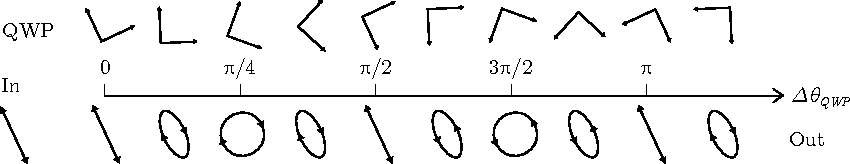
\includegraphics[scale=1.0]{./figures/background/chiroptics/QWP_in_out.pdf}
    \caption{\label{fig:background:Chirality:QWP}Output polarisation from a QWP at an angle $\Delta\theta_{QWP}$ to the input polarisation. The angle of the incident polarisation (and subsequent elliptical and linear outputs) can controlled by a half-wave plate.}
\end{figure}

Whereas linear birefringence results from structural anisotropy, a medium with structural \textit{chirality}, such as a chiral molecular system, can exhibit a similar dissymmetry in its interaction with LCP and RCP light. This leads to chiral-optical (chiroptical) effects, directly beneficial for both polarisation optics, and the characterisation of unknown chiral structures. The rest of this chapter discusses the physical origin of chiroptical effects relevant to this work, and the parameters used to characterise the interactions between chiral structures and light.


\section{Structural Chirality}\label{sec:background:Chirality:Structural}
In the simple case of a linear, isotropic medium, the macroscopic electromagnetic response of the material is described by the constitutive relations given in equation~\ref{eq:background:chirality:isotropicConstitutive}. These relate the material's internal electric displacement field $\bf{\tilde D}$ and magnetic field strength $\bf{\tilde H}$ to external electric and magnetic fields $\bf{\tilde E}$ and $\bf{\tilde B}$, where tildes denote complex values. Here, $\varepsilon$ and $\mu$ are complex scalars and correspond to the isotropic electric permittivity and magnetic permeability of the material.
\begin{equation}\label{eq:background:chirality:isotropicConstitutive}
	\begin{split}
        & \bf{\tilde D} = \tilde \varepsilon \bf{\tilde E} \\
        & \bf{\tilde B} = \tilde \mu \bf{\tilde H}
	\end{split}
\end{equation}
In the general case however, we cannot assume isotropy. Furthermore, $\bf{\tilde D}$ and $\bf{\tilde H}$ may depend on both $\bf{\tilde E}$ and $\bf{\tilde B}$ (magnetoelectric coupling). For a bi-anisotropic medium (anisotropic, with no-zero magnetoelectric coupling), the constitutive relations take the form of equation~\ref{eq:background:chirality:fullConstitutive}.\cite{Ishimaru2003, Capolino2009}. Here, $\bf{\tilde \varepsilon}$, $\bf{\tilde \mu}$, $\bf{\tilde \xi}$, and $\bf{\tilde \zeta}$ are $3 \times 3$ matrices due to the anisotropy of the material. $\bf{\tilde \xi}$, and $\bf{\tilde \zeta}$ are pseudo-scalars (behaving as scalars, but changing sign under parity inversion), and describe the magnetoelectric coupling.
\begin{equation}\label{eq:background:chirality:fullConstitutive}
    \begin{bmatrix}
        \bf{\tilde D} \\
        \bf{\tilde B}
    \end{bmatrix}
    =
    \begin{bmatrix}
        \bf{\tilde \varepsilon} & \bf{\tilde \xi} \\
        \bf{\tilde \zeta} & \bf{\tilde \mu}
    \end{bmatrix}
    \begin{bmatrix}
        \bf{\tilde E} \\
        \bf{\tilde H}
    \end{bmatrix}
\end{equation}
In the case of a non-gyrotropic material (exhibiting no magneto-optic rotation), equation~\ref{eq:background:chirality:fullConstitutive} has additional constraints, due to time-reversal symmetry, given in equation~\ref{eq:background:chirality:nongyroConstraints} \cite{Ishimaru2003}.
\begin{equation}\label{eq:background:chirality:nongyroConstraints}
    \begin{split}
        &[\bf{\tilde \xi}]^t = -[\bf{\tilde \zeta}] \\
        &[\bf{\tilde \varepsilon}]^t = [\bf{\tilde \varepsilon}] \\
        &[\bf{\tilde \mu}]^t = [\bf{\tilde \mu}]
    \end{split}
\end{equation}
The expressions shown in equation~\ref{eq:background:chirality:isotropicConstitutive} are a special case of equation~\ref{eq:background:chirality:fullConstitutive}, where no magneto-electric cross-coupling is present, so $\bf{\tilde \xi}=\bf{\tilde \zeta}=0$, and due to isotropy $\bf{\tilde \varepsilon}$ and $\bf{\tilde \mu}$ become scalars. 
In the case of a non-chiral anisotropic material, $\bf{\tilde \xi}=\bf{\tilde \zeta}=0$ however $\bf{\tilde \varepsilon}$ and $\bf{\tilde \mu}$ remain as matrices. Most relevant in this discussion however is the special case of a homogeneous bi-isotropic (isotropic chiral) medium. 
In this case the matrix components reduce to scalars, but all four components remain. The constraints given in equation~\ref{eq:background:chirality:nongyroConstraints} apply, and so we find that $\xi =-\zeta $.

There are several ways to write the remaining relations, including Post's relations~\cite{Capolino2009}, Born's relations~\cite{Lekner1999, Barnett2016} , and Tellegen's relations~\cite{Capolino2009,kong1986,lindell1994} (equation~\ref{eq:background:chirality:tellegensRelations}). Tellegen's relations will be used here, however the various forms are equivalent.
\begin{equation}\label{eq:background:chirality:tellegensRelations}
    \begin{bmatrix}
        \mathbf{\tilde D} \\
        \mathbf{\tilde B}
    \end{bmatrix}
    =
    \begin{bmatrix}
        \varepsilon_0 \tilde \varepsilon_r & i \tilde \kappa \sqrt{\mu_0 \varepsilon_0} \\
        -i \tilde \kappa \sqrt{\mu_0 \varepsilon_0} & \mu_0 \tilde \mu_r
    \end{bmatrix}
    \begin{bmatrix}
        \mathbf{\tilde E} \\
        \mathbf{\tilde H}
    \end{bmatrix}.
\end{equation}
Here, $\tilde \varepsilon_r$ and $\tilde \mu_r$ are the relative permittivity and permeability of the material respectively, and $\tilde \kappa$ is known as the structural ``chirality parameter''. In order to describe electromagnetic wave propagation through the chiral medium, we start by making use of the source-free time-harmonic Maxwell's equations in SI units convention. For a field oscillating at a frequency $\omega$, these take the form:
\begin{align}
    & \nabla \cdot \mathbf{\tilde D} = \nabla \cdot \mathbf{\tilde E} = 0 \label{eq:background:chirality:maxwellD}\\
    & \nabla \cdot \mathbf{\tilde B} = \nabla \cdot \mathbf{\tilde H} = 0 \label{eq:background:chirality:maxwellB}\\
    & \nabla \times \mathbf{\tilde E} = \frac{\partial \mathbf{\tilde B}}{\partial t} = i \omega \mathbf{\tilde B} \label{eq:background:chirality:maxwellE}\\
    & \nabla \times \mathbf{\tilde H} =  -\frac{\partial \mathbf{\tilde D}}{\partial t} = -i \omega \mathbf{\tilde D} \label{eq:background:chirality:maxwellH}.
\end{align}
For simplicity, equation~\ref{eq:background:chirality:tellegensRelations} can be rewritten in terms of $\varepsilon = \varepsilon_0 \tilde \varepsilon_r$, $\mu = \mu_0 \tilde \mu_r$, and $\gamma = \tilde \kappa \sqrt{\mu_0 \varepsilon_0}$ to give
\begin{align}
    & \mathbf{\tilde D} = \varepsilon \mathbf{\tilde E} + i \gamma \mathbf{\tilde H} \label{eq:background:chirality:tellegensSimplifiedD} \\
    & \mathbf{\tilde H} = \frac{1}{\mu}( \mathbf{\tilde B} + i \gamma \mathbf{\tilde E} ) \label{eq:background:chirality:tellegensSimplifiedH}.
\end{align}
Inserting equation~\ref{eq:background:chirality:maxwellE} into equation~\ref{eq:background:chirality:tellegensSimplifiedH} gives an expression for $\mathbf{\tilde H}$ eliminating all fields other than $\mathbf{\tilde E}$:
\begin{equation}\label{eq:background:chirality:HofE}
    \mathbf{\tilde H} = \frac{1}{\mu} \left( \frac{1}{i \omega} \nabla \times \mathbf{\tilde E} + i \gamma \mathbf{\tilde E} \right).
\end{equation}
Then, by equating expressions for $\mathbf{\tilde D}$ from equations~\ref{eq:background:chirality:maxwellH} and~\ref{eq:background:chirality:tellegensSimplifiedD} we obtain
\begin{equation}\label{eq:background:chirality:equatingD}
    \frac{i}{\omega} \nabla \times \mathbf{\tilde H} = \varepsilon \mathbf{\tilde E} + i \gamma \mathbf{\tilde H}.
\end{equation}
Substituting equation~\ref{eq:background:chirality:HofE} into equation~\ref{eq:background:chirality:equatingD} gives
\begin{equation}\label{eq:background:chirality:diffEfull}
    \frac{i}{\omega \mu} \nabla \times \left( \frac{1}{i \omega} \nabla \times \mathbf{\tilde E} + i \gamma \mathbf{\tilde E} \right) = \varepsilon \mathbf{\tilde E} + i \frac{\gamma}{\mu} \left( \frac{1}{i \omega} \nabla \times \mathbf{\tilde E} + i \gamma \mathbf{\tilde E} \right).
\end{equation}
For a \textit{homogeneous} isotropic chiral medium this can be simplified to obtain the following differential equation for the electric field:
\begin{equation}\label{eq:background:chirality:diffEreduced}
    \nabla \times (\nabla \times \mathbf{\tilde E}) - (\varepsilon \mu - \gamma^2)\omega^2 \mathbf{\tilde E} - 2 \omega \gamma \nabla \times \mathbf{\tilde E} = 0.
\end{equation}
By making use of the vector identity $\nabla \times (\nabla \times \mathbf{\tilde E}) = \nabla(\nabla \cdot \mathbf{\tilde E}) - \nabla^2 \mathbf{\tilde E}$ and equation~\ref{eq:background:chirality:maxwellD}, this is further simplified to give
\begin{equation}\label{eq:background:chirality:diffE}
    \nabla^2 \mathbf{\tilde E} + (\varepsilon \mu - \gamma^2)\omega^2 \mathbf{\tilde E} + 2 \omega \gamma \nabla \times \mathbf{\tilde E} = 0.
\end{equation}
Due to isotropy and homogeneity we can, without loss of generality, assume a monochromatic plane-wave solution propagating in the $z$ direction with a wavevector $k$ of the form
\begin{equation}
    \mathbf{\tilde E} = \begin{bmatrix}
        \tilde E_x \\
        \tilde E_y \\
        \tilde E_z
      \end{bmatrix} e^{i k z}
\end{equation}
where $\tilde E_x$, $\tilde E_y$, and $\tilde E_z$ are the complex scalar amplitudes of $x$, $y$, and $z$ components of the oscillating electric field respectively. The problem can be further simplified by noting that $\nabla \cdot \mathbf{\tilde E} = 0$ (equation~\ref{eq:background:chirality:maxwellD}), and therefore $\tilde E_z = 0$. Inserting the plane-wave solution into equation~\ref{eq:background:chirality:diffE}, and leaving in vector notation, gives:
\begin{equation}\label{eq:background:chirality:diffEvec}
    \nabla^2 \begin{bmatrix}\tilde E_x e^{i k z}\\ \tilde E_y e^{i k z} \\0 \end{bmatrix}+ (\varepsilon \mu - \gamma^2)\omega^2 \begin{bmatrix}\tilde E_x e^{i k z}\\ \tilde E_y e^{i k z} \\0 \end{bmatrix} + 2 \omega \gamma \nabla \times \begin{bmatrix}\tilde E_x e^{i k z}\\ \tilde E_y e^{i k z} \\0 \end{bmatrix} = 0.
\end{equation}
Expanding the del operator terms using
\begin{equation}
    \nabla^2 
    \begin{bmatrix}
        \tilde E_x e^{i k z}\\ 
        \tilde E_y e^{i k z} \\
        0 
    \end{bmatrix} 
    = 
    \begin{bmatrix} 
        \tilde E_x \\ 
        \tilde E_y \\ 
        0 
    \end{bmatrix} 
    (-k^2 e^{i k z}), \qquad
    \nabla \times
    \begin{bmatrix}
        \tilde E_x e^{i k z}\\ 
        \tilde E_y e^{i k z} \\
        0 
    \end{bmatrix} 
    = 
    \begin{bmatrix} 
        -\tilde E_y \\ 
        \tilde E_x \\ 
        0 
    \end{bmatrix} 
    (i k e^{i k z}) 
\end{equation}
reduces equation~\ref{eq:background:chirality:diffEvec} to
\begin{equation}\label{eq:background:chirality:waveEreduced}
    -k^2 \begin{bmatrix}\tilde E_x\\ \tilde E_y\end{bmatrix} e^{i k z} + (\varepsilon \mu - \gamma^2)\omega^2 \begin{bmatrix}\tilde E_x\\ \tilde E_y\end{bmatrix} e^{i k z} + 2 i \omega k \gamma \begin{bmatrix}\tilde E_x\\ -\tilde E_y\end{bmatrix} e^{i k z} = 0.
\end{equation}
Equation~\ref{eq:background:chirality:waveEreduced} can then be recast as an eigenproblem of the form $\underline{M}\mathbf{E} = 0$, specifically:
\begin{equation}
    \begin{bmatrix}
		(\varepsilon \mu - \gamma^2)\omega^2 -k^2  & -2 i \omega k \gamma \\ 
		2 i \omega k \gamma & (\varepsilon \mu - \gamma^2)\omega^2 -k^2
    \end{bmatrix}
    \begin{bmatrix} 
        \tilde E_x \\ 
        \tilde E_y
    \end{bmatrix} 
    = 0.
\end{equation}
This problem has nontrivial solutions only if 
\begin{equation}
    \mathrm{det}(\underline{M}) = 
    \begin{vmatrix}
        (\varepsilon \mu - \gamma^2)\omega^2 -k^2  & -2 i \omega k \gamma \\ 
		2 i \omega k \gamma & (\varepsilon \mu - \gamma^2)\omega^2 -k^2
    \end{vmatrix}    
    = 0.
\end{equation}
Finding the determinant of $\underline{M}$ gives
\begin{equation}
    \mathrm{det}(\underline{M}) = 
    \omega^4 (\gamma^2 - \varepsilon \mu)^2 - 2 k^2 \omega^2 (\gamma^2 + \varepsilon \mu) + k^4
    = 0.
\end{equation}
Solutions to this expression then directly yield the dispersion relations for light propagating through the medium:
\begin{equation}
    \begin{split}
        & k_{\pm} = \omega (\sqrt{\varepsilon \mu} \pm \gamma)
    \end{split}.
\end{equation}
In terms of the chirality parameter $\kappa$, these can be rewritten as
\begin{equation}\label{eq:background:chirality:kpmKappa}
    {k_\pm } = {k_0}\left( \sqrt {\tilde \mu_r \tilde \varepsilon_r} \pm \tilde \kappa  \right)
\end{equation}
where $k_0=\omega / c_0$ is the wave number in vacuum (and $c_0=1/\sqrt {{\mu _0}{\varepsilon _0}}$ is the speed of light in vacuum). The associated eigenwaves $\mathbf{\tilde E}_+$ and $\mathbf{\tilde E}_-$ are given by
\begin{equation}
    \mathbf{\tilde E}_{\pm} = \begin{bmatrix}\tilde E_x\\ \pm i \tilde E_y\end{bmatrix} e^{i k z}
\end{equation}
and correspond to right ($+$) and left ($-$) circularly polarised light respectively~\cite[\S 2.2]{Lekner1999}\cite{Chern2013}.
The refractive indices of the medium for propagating RCP and LCP light are therefore given by equation~\ref{eq:background:chirality:npmKappa}~\cite{Capolino2009, Qiu2008, Valev2013b}. 
\begin{equation}\label{eq:background:chirality:npmKappa}
    {\tilde n_ \pm } = \sqrt {\tilde \mu_r \tilde \varepsilon_r}  \pm \tilde \kappa
\end{equation}
Larger values of $\tilde \kappa$ lead to larger chiral dissymmetry: the difference in the optical response of a material to left- and right-circularly polarised light.
Additionally, for a sufficiently large value of $\tilde \kappa$, negative refractive index can be achieved for one direction of CPL.

\section{Chiroptical Effects}\label{sec:background:Chirality:Chiroptics}
Any material with a non-zero chirality parameter $\kappa$ will necessarily exhibit chiroptical effects dependent on its real and imaginary parts. As in section~\ref{sec:background:Chirality:Structural}, the real part of the refractive index of a medium $n$ describes the phase velocity of light propagating through the medium, and the imaginary part describes the absorption of light by the medium. From equation~\ref{eq:background:chirality:kpmKappa}, $\operatorname{Im}(\kappa)$ thus describes the differential \textit{absorption} of LCP and RCP light, known as circular dichroism (CD). 
\begin{figure}[htb!]
    \centering
    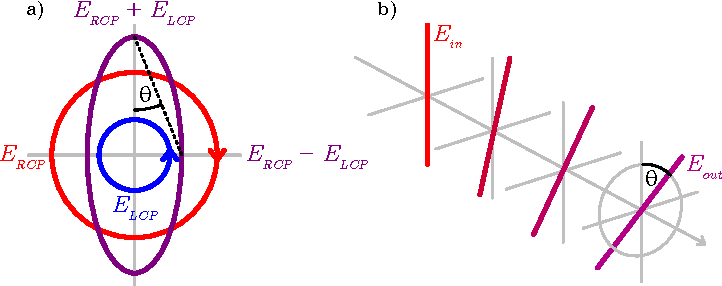
\includegraphics[scale=1.0]{./figures/background/chiroptics/cdor.pdf}
    \caption{\label{fig:background:Chirality:cdor}\textbf{a)} Schematic diagram of circular dichroism, characterised by the ellipticity ellipticity $\theta$ defined in terms of the field amplitudes of RCP and LCP light $E_{RCP}$ and $E_{LCP}$. The ellipticity is given by equation~\ref{eq:background:Chirality:CD}. \textbf{b)} Schematic diagram of optical rotation, showing linearly polarised light rotated by an angle $\theta$ throughout propagation through an optically active medium.}
\end{figure}
In linear optics, the circular dichroism at a particular wavelength of light is quantified by the ellipticity $\theta$, as defined by equation~\ref{eq:background:Chirality:CD}, and shown schematically in figure~\ref{fig:background:Chirality:cdor}a. 
\begin{equation}\label{eq:background:Chirality:CD}
    \theta = \arctan\left( \frac{E_{RCP} - E_{LCP}}{E_{RCP} + E_{LCP}} \right)
\end{equation} 
Here, $E_{RCP}$ and $E_{LCP}$ are the amplitudes of RCP and LCP light \textit{after} interaction with the chiral material. If $\operatorname{Im}(\kappa) = 0$, light can still be absorbed by the medium, but due to mirror symmetry, RCP and LCP light will be absorbed equally, and the CD as defined in equation~\ref{eq:background:Chirality:CD} is zero. For a non-zero $\operatorname{Im}(\kappa)$, $E_{RCP}$ and $E_{RCP}$ depend on both the magnitude of $\operatorname{Im}(\kappa)$, and the propagation length through the absorbing medium. If the propagation length is known, then circular dichroism can be used as a probe for the chirality parameter $\kappa$.
Correspondingly, $\operatorname{Re}(\kappa)$ describes the differential \textit{phase velocity} for LCP and RCP light. Since linearly polarised light can be represented by a superposition of equal-amplitude LCP and RCP waves, a linearly polarised wave, of vacuum wavevector $k_z$ propagating through a medium with RCP and LCP refractive indices given by $n_+$ and $n_-$ respectively, is described by equation~\ref{eq:background:Chirality:OR}~\cite[\S 8.10]{Hecht2013}.
\begin{equation}\label{eq:background:Chirality:OR}
    \begin{split}
        \mathbf{E} = E_0 \cos(k_z (\frac{n_+ + n_-}{2})z -\omega t &) \left[ \mathbf{\hat{x}} \cos(k_z (\frac{n_+ - n_-}{2})z ) \right. \\
        & \left. + \mathbf{\hat{y}} \sin(k_z (\frac{n_+ - n_-}{2}) z)\right]
    \end{split}
\end{equation}
At any point in time throughout propagation, the RCP and LCP components are oscillating in phase and with equal amplitudes, meaning that the resultant wave remains linearly polarised. However, the orientation of the linear polarisation will rotate throughout propagation, with the rate and direction of rotation depending on the magnitude and sign of $n_+ - n_-$ respectively. This effect is the chiral counterpart to birefringence, where orthogonal \textit{linear} polarisations exhibit different phase velocities. It is thus known as ``circular birefringence''. In the case of linear birefringence, optical rotation is achieved by utilising a fixed $\lambda/2$ phase shift, and rotating the mediums fast axis relative to the incident polarisation to control the angle of rotation. Conversely, a material exhibiting circular birefringence will rotate linearly polarised light continuously during propagation, shown schematically in figure~\ref{fig:background:Chirality:cdor}b. Therefore, the resulting angle of optical rotation ($\theta$ in figure~\ref{fig:background:Chirality:cdor}b) depends on both the strength of circular birefringence, and the propagation length through the medium. Optical rotation can therefore also be used as a method to characterise the chirality parameter $\kappa$ of the material. Collectively, circular dichroism and optical rotation are referred to as ``optical activity''.

Generally, in real materials the refractive index $n$ is strongly wavelength-dependent. The wavelength-dependent refractive index $n(\lambda)$ includes contributions from the wavelength-dependent structural chirality parameter $\kappa(\lambda)$. The dependence of $n(\lambda)$ on $\kappa(\lambda)$ directly leads to wavelength-dependent CD and OR, the latter specifically known as optical rotatory dispersion (ORD). CD spectra can be measured by taking extinction spectra LCP and RCP light propagating through the material, and applying equation~\ref{eq:background:Chirality:CD} at each wavelength, where $E_{RCP}$ and $E_{RCP}$ are the amplitudes of the transmitted RCP and LCP light respectively. Similarly, ORD spectra can be obtained by propagating linearly polarised light through the medium, and detecting the intensity of transmitted light through a rotatable analysing polariser. The analyser angle transmitting maximum intensity gives the resulting angle of polarisation, which can be compared to the incident polarisation to find the angle of optical rotation. Again, this can be taken at each wavelength to construct an ORD spectrum. It is important to reiterate however, that OR and CD depend on the real and imaginary parts of the same complex refractive index $n$. CD and ORD spectra are thus intrinsically linked by the Kramers-Kronig transforms: each can be obtained from the other, and they fundamentally contain the same information. 


\subsection{Chiroptical Effects from Extrinsic Chirality}\label{sec:background:Chirality:extrinsic}
It is possible to obtain a chiroptical response from structures that exhibit neither 3D nor planar chirality. Instead, chirality is introduced by the geometry of the experiment itself; the wave-vector, the surface normal and the direction of curvature on the structure form a chiral triad. 
The fundamental mechanism for this optical activity is shown in figure~\ref{fig:background:Chirality:extrinsic}. When illuminated at normal incidence, the structure geometry remains unchanged when projected onto the transverse plane of the incident light (figure~\ref{fig:background:Chirality:extrinsic} left). However, when the sample is illuminated at an oblique angle the projection of the structure geometry onto the transverse plane of incident light becomes distorted. Under inversion, the structure's projection can no longer be superimposed onto itself by in-plane rotation, and is therefore planar chiral, as shown in figure~\ref{fig:background:Chirality:extrinsic} (right). 
If optical activity due to extrinsic chirality is measured at an oblique angle of incidence $\phi$, then the chiroptical response should change sign when measured at an angle of incidence of $-\phi$. That is, any measured circular dichroism will reverse sign, and any optical rotation will rotate in the opposite direction. This can perhaps be more intuitively understood by considering the geometry shown in figure~\ref{fig:background:Chirality:extrinsic}. The projection of the structure's mirror image at oblique incidence is identical to its own projection at the opposite angle of incidence. By reversing the angle of incidence, the chirality of the experimental geometry is reversed, and any chiroptical effects will correspondingly change sign.
\begin{figure}[htb!]
    \centering
    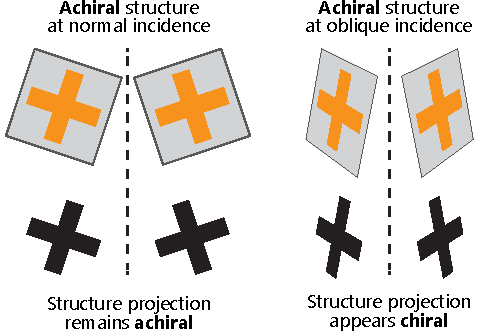
\includegraphics[scale=1.0]{./figures/background/chiroptics/extrinsic_chirality.pdf}
    \caption{\label{fig:background:Chirality:extrinsic}Schematic representation of extrinsic chirality in an achiral structure.}
\end{figure}
Plum et al. showed that asymmetric transmission (circular difference) can occur in any structure whose projection onto the transverse plane of incident light is 2-dimensionally chiral and anisotropic~\cite{Plum2011}. It is therefore possible to achieve chiroptical effects utilising geometrically simpler structures than those that are intrinsically chiral.

For applications requiring manipulation of light polarisation, such as optical rotation or circular dichroism, it is perfectly possible to use extrinsic instead of intrinsic chirality. An early study by Plum et al., for example, measured a chiroptical response from achiral split-ring structures at microwave wavelengths~\cite{Plum2009c}. These structures were shown to exhibit both circular dichroism and optical rotation when illuminated at oblique incidence. At normal incidence, no significant optical activity was measured for either structure. The circular birefringence resulted in rotation of linear polarisation exceeding $\SI{60}{\degree}$ for microwaves. Later observations, directly comparing extrinsic and intrinsic chirality, confirmed that the former can yield significantly stronger response~\cite{Maoz2012a}. 
More recent work has pushed towards optical-wavelength chiroptical responses due to extrinsic chirality.
Cao et al. demonstrated, experimentally and computationally, strong circular dichroism in the mid-IR region ($\approx\SI{2.4}{\micro\m}$), resulting from extrinsic chirality in achiral metallic nanostructures~\cite{Cao2014}. Both enantiomorphs of the structure can be obtained by tilting the sample to opposite angles. This fact, it is suggested, can be utilised to simplify experiments requiring both enantiomers of a nanostructure, by removing the need to fabricate two separate structures.
More recently, Belardini et al. have demonstrated strong chiroptical effects at \textit{optical} wavelengths from a surface of tilted nanowires~\cite{Belardini2016}. It was shown that upon rotating the sample by $\SI{180}{\degree}$, both the circular dichroism and angle of optical rotation change sign, as expected for extrinsic chirality. 
The same work also reported that extrinsic chirality affects nonlinear chiroptical measurements (discussed further in section~\ref{sec:background:NonlinearOptics}) in a similar way. Nonlinear chiroptical measurements were taken as a function of the angle of incidence of light, for opposite orientations of the nanowires. As expected, the opposite orientations resulted in a reversal of the nonlinear chiroptical response. Additional work demonstrated the same dependency of the nonlinear chiroptical response on the angle of optical incidence, and that extrinsic chirality is induced by the relative angle between the light and the surface normal~\cite{Belardini2015}.

The relative simplicity of fabrication for achiral nanostructures could open the field to more readily available and easier to mass-produce geometries. The key here would be to consider the experimental geometry as a whole. However, in experiments aiming to characterise the chirality of materials at oblique incidence, contributions to measurable chiroptical effects from extrinsic chirality can complicate analysis. Importantly, extrinsic chirality can be identified by comparing the symmetry of contributions from intrinsic and extrinsic chirality. Chiroptical effects originating from true intrinsic chirality should be invariant upon rotation of the angle of incidence. Conversely, contributions originating from extrinsic chirality will reverse as the angle of incidence changes sign.


\subsection{Chiroptical Effects from Anisotropy}\label{sec:background:Chirality:anisotropy}

It was shown earlier in section~\ref{sec:background:Chirality} that the rotation and circularly polarisation of linearly polarised light can occur in achiral, anisotropic materials.
Despite applications in polarisation optics, structural anisotropy raises issues when characterising chiral systems. 
Within stereochemistry, chiroptical analysis historically tends to occur in isotropic, homogenous liquid molecular systems~\cite{Berova2012a}. In these cases, the anisotropy of individual molecules has no significant effect on the macroscopically measured optical activity. This is due to the 3-dimensional averaging out of anisotropy for a large number of randomly oriented molecules. 
However, the work in this thesis makes use of planar metallic ``nanomaterials'', discussed in greater depth in section~\ref{sec:background:Plasmonics}. These nanomaterials are commonly fabricated by patterning metallic inclusions onto a 2-dimensional surface, and so typically cannot be isotropically arranged. 

Previous work has demonstrated that, towards the nanoscale, achiral, anisotropic structures can locally generate circularly polarised light~\cite{Hashiyada2018}. Conversely, a linearly birefringent material can convert circularly polarised light to linearly polarised light. 
Such birefringent materials can also exhibit linear dichroism (a difference in the absorption of orthogonal linearly polarisations). This can lead to an apparent circular dichroism, actually the combined effect of linear birefringence and linear dichroism. Likewise, the operation of half-wave plates demonstrates the ability for anisotropic, achiral media to result in significant optical rotation of linearly polarised light. 
When characterising the chirality of anisotropic structures, there is thus a prevailing need for experimental techniques capable of disentangling contributions from anisotropy and intrinsic chirality. 
Fortunately, chiroptical contributions from anisotropy can also be identified with symmetry considerations. Any chiroptical effects measured due to an isotropic structure's intrinsic chirality will be invariant under structure rotation. Conversely, chiroptical effects originating exclusively from anisotropy will necessarily vary as the structure is rotated, reversing sign upon $\SI{90}{\degree}$ rotation normal to the fast and slow axis of the material. However, this periodic sign change is not strictly necessary in structures that exhibit both intrinsic or extrinsic chirality \textit{and} structural anisotropy. In these cases, the two contributions are effectively competing, and complex chiroptical behaviour can emerge~\cite{Hooper2017}. Isolating the structural chirality from anisotropy and extrinsic chirality is therefore challenging, especially in planar nanomaterials which are often highly anisotropic. In sections~\ref{sec:results:OAinPlanarNanohelices} and~\ref{sec:results:HRS} two methods of experimentally isolating the intrinsic chirality of metallic nanomaterials are explored.


\section{Optical Chirality and ``Superchiral'' Light}\label{sec:background:Chirality:opticalchirality}
The interaction between a chiral molecule and a chiral electromagnetic field is expected to exhibit a dissymmetry, in that each ``handedness'' of a chiral field should interact differently with a chiral molecule or nanostructure. A field with a shorter chiral pitch, the distance over which the polarisation vector completes a $\SI{360}{\degree}$ twist, will exhibit a stronger interaction dissymmetry than a less twisted field. It had long been thought that the maximum possible chiral dissymmetry is obtained for a perfectly circularly polarised monochromatic field, however in 2010 Tang and Cohen proposed a setup in which the dissymmetry exceeds that of CPL (referred to as ``superchiral light'') at the nodes of a chiral standing wave.~\cite{Tang2010}
The strength of the field chirality can be quantified by Lipkin's 00-zilch density~\cite{Lipkin1964} referred to by Tang and Cohen as the ``optical chirality'' $C$ as defined in equation~\ref{eq:background:chirality:opticalchirality}. This quantity is a time-even pseudo-scalar, as would be expected for a measure of true chirality.
\begin{equation} \label{eq:background:chirality:opticalchirality}
    \begin{split}
        C = &\frac{\varepsilon_0 }{2}{\bf{\tilde E}} \cdot (\nabla  \times {\bf{\tilde E}}) + \frac{1}{{2\mu _0}}{\bf{\tilde B}} \cdot (\nabla  \times {\bf{\tilde B}}) \\
        = &- \frac{{{\varepsilon _0}\omega }}{2} \operatorname{Im}[ \bf{\tilde E}(\bf{r}) \cdot \bf{\tilde B}(\bf{r}) ]
    \end{split}
\end{equation}
Here, $\bf{\tilde E}$ and $\bf{\tilde B}$ denote the complex electric and magnetic field amplitudes respectively. This quantity describes the angular momentum of the curl of the optical field~\cite{Cameron2012a} and is a conserved property of the field. Tang and Cohen showed that the enantioselectivity of optical excitation of a molecule is highly dependent on $C$, and so it stands that such a superchiral field can lead to significant enhancement of the enantioselective excitation of chiral molecules.

The general microscopic response of a chiral molecule to a monochromatic electromagnetic field is described by an induced electric dipole moment $\mathbf{\tilde p}$ and magnetic dipole moment $\mathbf{\tilde m}$ as in equation~\ref{eq:background:chirality:tangDipole}.
\begin{equation}
    \label{eq:background:chirality:tangDipole}
    \begin{split}
        &{\bf{\tilde p}} = {{\tilde \alpha }_{ee}}{\bf{\tilde E}} - i{{\tilde \alpha }_{em}}{\bf{\tilde B}} \\
        &{\bf{\tilde m}} = i{{\tilde \alpha }_{em}}{\bf{\tilde E}} + {{\tilde \alpha }_{mm}}{\bf{\tilde B}}
    \end{split}
\end{equation}
Here, $\tilde{\alpha}_{ee}$ and $\tilde{\alpha}_{mm}$ correspond to $\tilde{\alpha}$ and $\tilde{\chi}$ in references~\cite{Tang2010} and~\cite{Choi2012}, 
$\alpha_{ee}$ is the electric polarisability, and $\alpha_{mm}$ is the magnetic susceptibility. $\tilde{\alpha}_{em}$ is the mixed magneto-electric polarisability and is directly related to the material chirality parameter $\kappa$ (section~\ref{sec:background:Chirality:Structural}).
Physical quantities are obtained from the real parts of equation (14). For an incident electric field $\mathbf{\tilde{E}}=\mathbf{\tilde{E}}_{0}{e}^{-i\omega t}$ and $\mathbf{\tilde{B}}=\mathbf{\tilde{B}}_{0}{e}^{-i\omega t}$ the rate of excitation of a molecule from right ($+$) and left ($-$) CPL is given by equation~\ref{eq:background:chirality:Aplusminus} \cite{Tang2010, Choi2012}.

\begin{equation} \label{eq:background:chirality:Aplusminus}
    {A^ \pm } = 
    \frac{\omega }{2}{\left\langle {{\bf{E}} \cdot {\bf{\dot p}} + {\bf{B}} \cdot {\bf{\dot m}}} \right\rangle _t} = 
    \frac{\omega }{2}{\mathop{\rm Im}\nolimits} ({{\bf{\tilde E}}^ * } \cdot {\bf{\tilde p}} + {{\bf{\tilde B}}^ * } \cdot {\bf{\tilde m}})
\end{equation}
Substituting equation~\ref{eq:background:chirality:tangDipole} into equation~\ref{eq:background:chirality:Aplusminus} leads to equation~\ref{eq:background:chirality:AplusminusFull}, which can be rewritten in terms of the generalised optical chirality $C$ to give equation~\ref{eq:background:chirality:AplusminusC}~\cite{Choi2012}. Here ${\tilde \alpha }_{em}''=\operatorname{Im}({\tilde \alpha }_{em})$.
\begin{equation} \label{eq:background:chirality:AplusminusFull}
    {A^ \pm } = \frac{\omega }{2}({\tilde \alpha ''_{ee}}{\left| {{\bf{\tilde E}}} \right|^2} + {\tilde \alpha ''_{mm}}{\left| {{\bf{\tilde B}}} \right|^2}) \pm {\tilde \alpha }_{em}''\omega {\mathop{\rm Im}\nolimits} ({{\bf{\tilde E}}^ * } \cdot {\bf{\tilde B}})
\end{equation}
\begin{equation} \label{eq:background:chirality:AplusminusC}
    {A^ \pm } \simeq \frac{\omega }{2}({\tilde \alpha ''_{ee}}{\left| {{\bf{\tilde E}}} \right|^2} + {\tilde \alpha ''_{mm}}{\left| {{\bf{\tilde B}}} \right|^2}) \pm {\tilde \alpha }_{em}''\frac{2}{\varepsilon }C
\end{equation}
The time averaged electric and magnetic energy densities ${{\left\langle {{U}_{E}} \right\rangle }_{t}}=\tfrac{\varepsilon }{4}{{\left| {\mathbf{\tilde{E}}} \right|}^{2}}$ and ${{\left\langle {{U}_{B}} \right\rangle }_{t}}=\tfrac{1}{4\mu }{{\left| {\mathbf{\tilde{B}}} \right|}^{2}}$  can be introduced here, and substituted into equation~\ref{eq:background:chirality:AplusminusC} to give the rate of excitation in terms of energy density as in equation~\ref{eq:background:chirality:AplusminusU}. 
\begin{equation}\label{eq:background:chirality:AplusminusU}
    \begin{split}
        & {A^ \pm } \simeq \frac{2}{\varepsilon }{{\tilde \alpha ''}_{ee}}\omega \left( {{{\left\langle {{U_E}} \right\rangle }_t} + \gamma {{\left\langle {{U_B}} \right\rangle }_t}} \right) \pm {\tilde \alpha }_{em}''\frac{2}{\varepsilon }C \\
        & \gamma  = \frac{{{{\tilde \alpha ''}_{mm}}}}{{{{\tilde \alpha ''}_{ee}}}}\varepsilon \mu  = \frac{{{{\tilde \alpha ''}_{mm}}}}{{{{\tilde \alpha ''}_{ee}}}}\frac{{{n^2}}}{{{c^2}}}
    \end{split}
\end{equation}
We can now define the dissymmetry factor $g$ of the chiroptical interaction by equation~\ref{eq:background:chirality:dissymmetryA}.
\begin{equation}\label{eq:background:chirality:dissymmetryA}
    g = \frac{{{A^ + } - {A^ - }}}{\frac{1}{2}({A^ + } + {A^ - })}
\end{equation}
In Tang and Cohen's proposal~\cite{Tang2010} the magnetic field was disregarded as negligible. Under this assumption, the dissymmetry factor is found to be 
\begin{equation}\label{eq:background:chirality:dissymmetryG}
    g =  - \frac{{{\tilde \alpha }_{em}''}}{{\tilde \alpha ''}_{ee}}\frac{{2C}}{{\omega {{\left\langle {{U_E}} \right\rangle }_t}}}
\end{equation}
Note that under this approximation, the dissymmetry factor splits into properties of the molecule only (${{\tilde \alpha }_{em}''}/{{\alpha }''}_{ee}$) and properties of the field only (${2C}/{\omega {{\left\langle {{U}_{E}} \right\rangle }_{t}}}$), however in the general case the dissymmetry factor cannot be separated in this way and is significantly more complex~\cite{Choi2012}.
The full expression accounting for magnetic energy density can be simplified by assuming a small dissymmetry factor such that $n_{+} \approx n_{-}$, to give equation~\ref{eq:background:chirality:dissymmetryFull}.~\cite{Choi2012}
\begin{equation}\label{eq:background:chirality:dissymmetryFull}
    g =  - \frac{{\tilde \alpha ''}_{em}}{{{\tilde \alpha ''}_{ee}}}\frac{{2C}}{{\omega [{{\left\langle {{U_E}} \right\rangle }_t} + \gamma {{\left\langle {{U_B}} \right\rangle }_t}]}}
\end{equation}
The limitation in chiroptical enhancement is now clear: in regions of low electric energy density, the magnetic energy density is maximised and should not be considered negligible. The $\gamma$ term in equation~\ref{eq:background:chirality:dissymmetryFull} is then the key limiting factor for the dissymmetry enhancement. The energy density terms in the denominator can no longer be reduced to arbitrarily small values in order to continually increase chiral dissymmetry. However, the chiral dissymmetry can still be increased by reducing the total electromagnetic energy density, increasing the structural chirality parameter of the medium, and increasing optical chirality $C$ of the electromagnetic field. 

Despite these limitations, Tang and Cohen experimentally verified enhanced chiral dissymmetry using superchiral nodes on a standing wave, as previously proposed. By comparing the fluorescence emission of chiral and achiral molecular layers under left- and right-polarised superchiral standing waves, they demonstrated an $11 \times$ dissymmetry enhancement compared to circularly polarised light~\cite{Tang2011}. This experimental configuration has clear practical limitations however, in that the target sample must be positioned at, or near, a node of a standing wave. Slight positional deviations of the sample, or the partially reflecting mirror, could easily result in the sample entering an anti-node, at which the optical chirality is minimised. To alleviate this limitation, experimental configurations have been proposed that fix the positioning of the standing wave, and the sample surface. Rather than using a partially reflective mirror to generate a standing wave, periodic photonic crystal structures have been used to form Bloch waves, which can lead to superchiral nodes at fixed positions through the photonic crystal structure~\cite{Sinibaldi2014, Pellegrini2017, Pellegrini2018}. By designing the structure and angle of optical incidence such that a node of high optical chirality occurs at the termination surface of the structure, chiral fields can be formed over large surface areas, used for sensing and characterisation of molecules attached to the material surface~\cite{Sinibaldi2014, Pellegrini2017}. These superchiral Bloch waves have been used to demonstrate two orders of magnitude increase in circular dichroism signal compared to probing with circularly polarised light~\cite{Pellegrini2017}.
Typically however, a more common method of experimentally realising superchiral light is the use of plasmonic nanomaterials, capable of generating periodic small regions of high optical chirality at the surface of a quasi-2-dimensional material. This is discussed further in section~\ref{sec:background:Plasmonics:superchiral}.


\section{Conclusions}

Across a wide range of research fields, chirality, the lack of mirror symmetry, is a key structural property, especially prevalent in biomolecular systems. Particularly, many pharmaceutical drugs are chiral, with enantiomers often exhibiting dramatically different medical effects.
Because of this, chiral optical (chiroptical) effects have become a widespread method for characterising the structural properties of complex molecular systems.
We have shown that structural anisotropy can be utilised to form chiral polarisation states of light, which can in turn be used to directly probe material chirality.
By considering the propagation of light through a medium exhibiting coupling between induced electric and magnetic dipoles, we have shown that left- and right-circularly polarised light will propagate through a chiral medium with different refractive indices. This chiral dissymmetry directly leads to circular dichroism, and optical rotation, two measurable probes of the real and imaginary parts of the chiral medium's refractive index.
In section~\ref{sec:background:Chirality:opticalchirality}, it was shown that, perhaps contrary to intuition, pure circularly polarised light does not necessarily lead to the strongest chiral dissymmetry. In fact, by interfering circularly polarised fields, the nodes of an elliptically polarised standing wave can exhibit a twisted field gradient stronger than that of CPL. This has allowed for molecular chiroptical measurements with significantly greater sensitivity than those undertaken with pure circularly polarised light.
As well as ``superchiral'' configurations, enhanced chiroptical sensitivity has been demonstrated by making use of nonlinear optics; an extremely symmetry-sensitive frequency conversion effect within media driven by intense electromagnetic fields. The following section discusses the microscopic origin of nonlinear scattering, the macroscopic descriptions of nonlinear media, and the symmetry properties of second-harmonic generation in particular, for use in chiroptical characterisation measurements.